\chapter{Background}

\section{Laser Trapped-Ion Experiment}

Trapped-ion quantum systems have emerged as a leading candidate for quantum computing platforms due to their outstanding coherence times, high-fidelity quantum gates, and promising scalability. In trapped-ion systems, charged atoms confined by electric fields are precisely controlled and manipulated using laser beams. These lasers serve instrumental roles, including initializing quantum states, implementing quantum gates, and performing state measurements \cite{naturequantuminfo}. 

However, traditional approaches for optical hardware tend to be bulky, expensive, and power-intensive, posing severe limitations on scalability. As the number of qubits in a trapped-ion quantum computing system grows, these challenges become more pronounced \cite{photonicreview}. Compact, efficient, and rapid modulation capabilities are thus needed to scale quantum computing platforms beyond small-scale demonstrations.

Recent advancements in photonic integrated circuits (PICs) have substantially addressed these challenges \cite{apic}. These PICs are miniaturized, enabling direct integration with ion-trap chips, thereby dramatically reducing optical losses, system complexity, and the overall footprint. Crucially, integrated modulators facilitate modulation at very high speeds—on the order of nanoseconds—which matches the stringent timing requirements of quantum operations \cite{naturequantuminfo}.

To fully utilize the capabilities of these advanced PICs, corresponding electronic control systems capable of generating precisely timed, flexible modulation signals at around 100 MHz resolution are necessary. The 100 MHz resolution provided by our system ensures that the modulation signals can be precisely timed and shaped, directly corresponding to the stringent timing requirements of quantum gates that often operate on microsecond timescales. Having 32 synchronous dynamic voltage channels is necessary because it allows the simultaneous manipulation of multiple qubits with coherent precision. The precise synchronization of these channels ensures minimal timing jitter and improved gate fidelity, which is indispensable for scaling quantum computing systems \cite{manychanfpgactrlsys}.

\section{Hardware Description}\label{sec:bg_hw}
% TODO: Diagram of the board/system
To meet the demands of advanced control electronics, this project utilizes a Field Programmable Gate Array (FPGA). FPGAs excel at high-speed, low-latency parallel processing, enabling the simultaneous control of multiple channels and the implementation of flexible, efficient digital signal processing algorithms. These capabilities make FPGAs particularly suited for managing complex experimental setups that demand precise timing and real-time adaptability. This project employs the Xilinx Zynq UltraScale+ ZCU102 Evaluation Board, a platform chosen for its remarkable computational resources and flexible high-speed interfacing capabilities.

The ZCU102 board (\autoref{fig:fpga_diagram}) is integral for generating precise modulation signals required by quantum lasers. It features a range of peripherals, including PMOD interfaces that support low-speed digital-to-analog converters (DACs) via SPI protocols, and two FMC HPC connectors for high-speed DACs. The core of this FPGA platform is the Xilinx Zynq architecture, which combines a Processing System (PS) with Programmable Logic (PL) \cite{XilinxUG1182}.

\begin{figure}[ht]
    \centering
    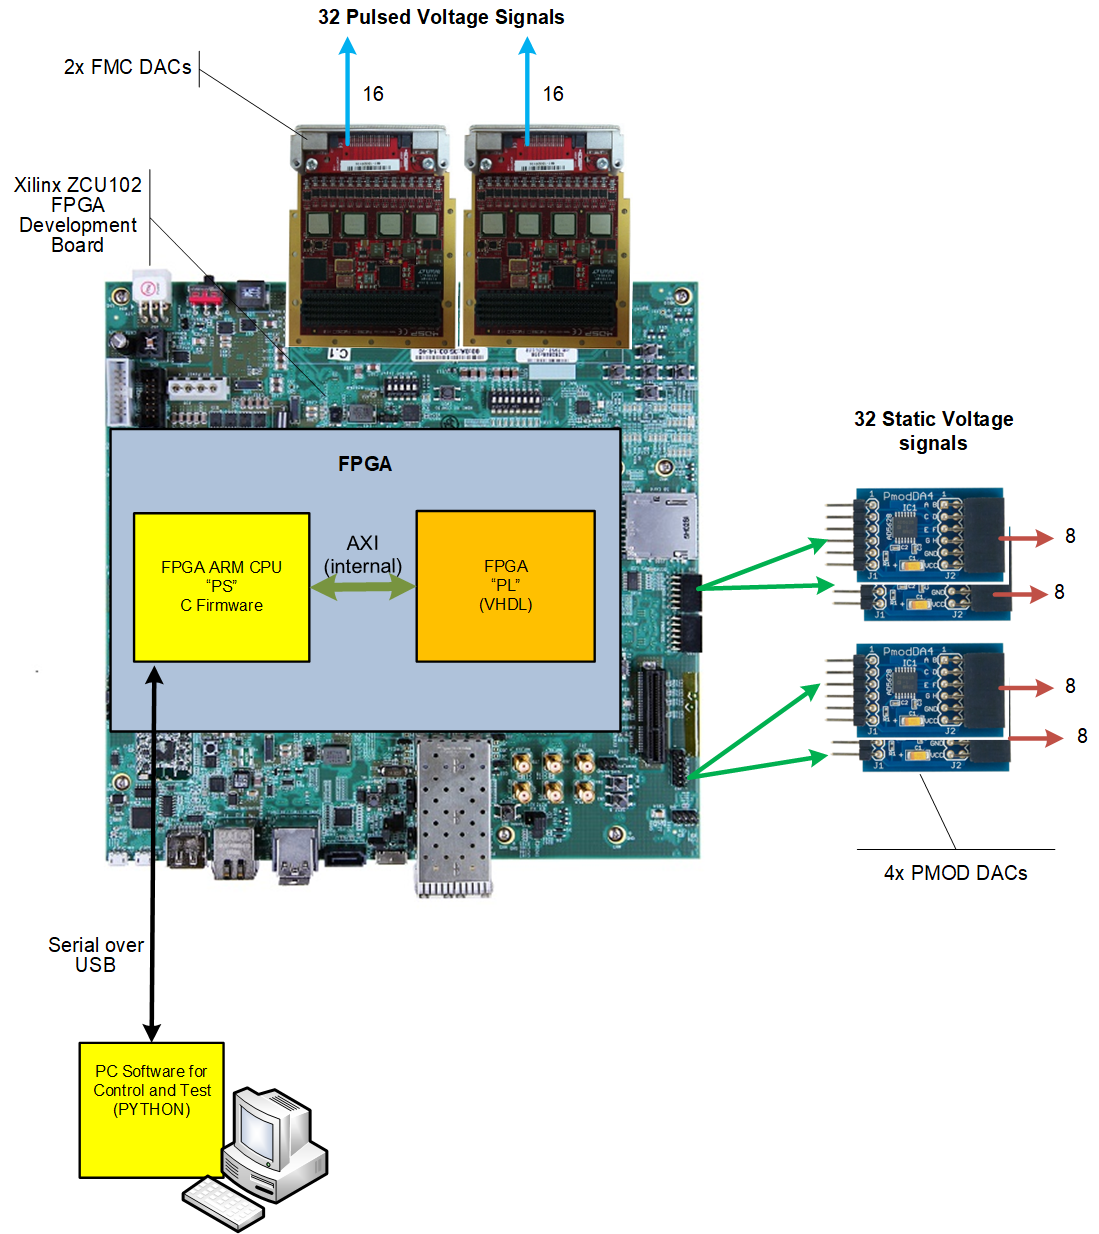
\includegraphics[width=0.80\linewidth]{figures/board.png}
    \caption{The FPGA board with necessary peripherals.}
    \label{fig:fpga_diagram}
\end{figure}

The PS is powered by a quad-core Arm\textsuperscript{\textregistered} Cortex\textsuperscript{\textregistered}-A53 processor, capable of running real-time processing applications. It incorporates multiple peripherals, such as DDR4 memory for application storage and an Advanced eXtensible Interface (AXI) that connects the PS to other components, including the programmable logic. The PL, which is the FPGA itself, contains logic cells, flip-flops, and block RAMs (BRAM) \cite{XilinxUG1182}. It provides ample capacity for storing intermediate data.

This project leverages programmable logic to build custom hardware designs that serve the unique demands of quantum laser experiments. The FPGA's dedicated logic circuits and integrated high-speed interfaces enable quick, reliable communication with external modules. This capability maintains accurate control and precise timing. General-purpose I/O options, such as PMOD and FMC connectors, further simplify the experimental setup. These connectors offer flexible interfacing, allowing for both low-speed and high-speed connections that scale to the experiment's complexity without sacrificing performance.

In addition to the hardware features, a Python interface abstracts the low-level hardware details, streamlines testing, and integration with the FPGA platform. Indicated in \autoref{fig:fpga_diagram}, a custom C-based program running in the processing system translates Python-generated commands into data that the FPGA can efficiently process. This layered approach bridges high-level control with low-level hardware performance, ensuring that experimental algorithms and rapid prototyping can be achieved.

\section{Pulse Sequence}\label{sec:hw_pulse}

In high-fidelity quantum computing and atomic manipulation, pulsed sequences are pivotal for delivering precise, accurate, and stable outputs to photonic integrated circuits \cite{apic}. These laser pulses (\autoref{fig:pulse_seq}) are designed with a controlled shape that consists of three distinct phases: rise, sustain, and fall. Each phase ensures quantum operations are performed reliably.

\begin{figure}[h]
    \setlength{\abovecaptionskip}{5pt}    % Reduces space above caption
    \setlength{\belowcaptionskip}{5pt}    % Reduces space below caption
    \centering
    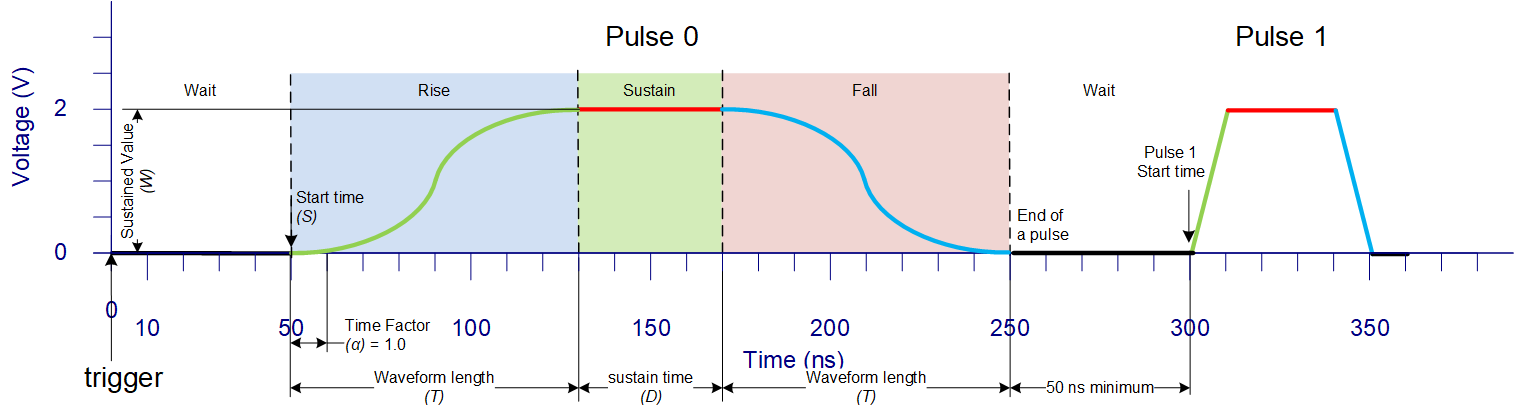
\includegraphics[width=1\linewidth]{figures/2.1.png}
    \caption{Example of the pulse sequence. Both the time and gain factors are set to 1}
    \label{fig:pulse_seq}
\end{figure}

During the rise phase, the laser intensity increases to its target level. A well-controlled rise minimizes errors and ensures that the experiment operate exactly when needed. The sustain phase follows, during which the laser maintains a constant optical intensity. This steady state is paramount because any fluctuation can compromise the fidelity of quantum gates by introducing operational errors \cite{naturequantuminfo}. Finally, the fall phase allows the laser power to decrease smoothly. Maintaining symmetry between the rise and fall phases is critical for consistency and repeatability. In this design, the fall essentially becomes the mirror image of the rise. The rise is a programmable waveform pattern, while the sustain is a flat region with programmable length. 
% The user stores the waveform values and pulse configurations in the FPGA's memory.
% TODO: this sounds better than the other version?
In addition, user settings specify additional parameters such as start time, sustain time, and waveform length, as described in \autoref{fig:pulse_seq}. These configurations enable the module to adjust pulse characteristics programmatically without redefining the waveforms. In many cases, a pulse is produced by scaling a common base waveform using programmable factors for both time and amplitude. However, when a pulse sequence includes pulses with different time and amplitude features, the configuration selects the distinct waveforms for each pulse. This approach ensures accurate and flexible control over the behavior of the entire sequence. 

\begin{figure}[ht]
    \setlength{\abovecaptionskip}{5pt}    % Reduces space above caption
    \setlength{\belowcaptionskip}{5pt}    % Reduces space below caption
    \centering
    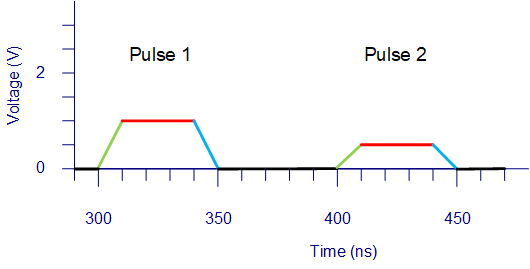
\includegraphics[width=0.7\linewidth]{figures/3.1.1.png}
    \caption{Two pulses with pulse 2 having half the amplitude of pulse 1.}
    \label{fig:gain_scale_example}
\end{figure}

For instance, the rising edge of pulse 0 in \autoref{fig:pulse_seq} follows a curved profile while pulse 1 increases linearly. Since these profiles cannot be interconverted by scaling alone, the user must define two unique waveforms and assign each to the respective pulse configurations. Furthermore, suppose a subsequent pulse, such as pulse 2, is intended to have half the amplitude of pulse 1 while retaining similar waveform characteristics (\autoref{fig:gain_scale_example}). In that case, the configuration should specify that pulse 2 uses the waveform of pulse 1 with a gain factor of 0.5. This structured configuration approach allows the module to adjust pulse characteristics without redefining fundamental waveforms, ensuring precise control over the entire sequence's behavior.

\begin{table}[ht]
    \setlength{\abovecaptionskip}{5pt}    % Reduces space above caption
    \setlength{\belowcaptionskip}{5pt}    % Reduces space below caption
    \centering
    \caption{A single pulse's output at various time}
    \begin{tabularx}{\textwidth}{|X|c|X|}
        \hline
        Time & Phase & Output \\
        \hline
        0&Wait&0\\
        \hline
        \multicolumn{3}{|c|}{\vdots}\\
        \hline
        $S_0-1$&Wait&0\\
        \hline
        $S_0$&Rise&$A_0f_0(0)$\\
        \hline
        $S_0+\alpha$&Rise&$A_0f_0(\frac{\alpha}{T_0})$\\
        \hline
        \multicolumn{3}{|c|}{\vdots}\\
        \hline
        $S_0+T_0$&Rise&$A_0f_0(\frac{T_0-1}{T_0})$\\
        \hline
        $S_0+T_0+1$&Sustain&$W_0$\\
        \hline
        \multicolumn{3}{|c|}{\vdots}\\
        \hline
        $S_0+T_0+D_0$&Sustain&$W_0$\\
        \hline
        $S_0+T_0+D_0+1$&Fall&$A_0f_0(\frac{T_0-1}{T_0})$\\
        \hline
        \multicolumn{3}{|c|}{\vdots}\\
        \hline
        $S_0+T_0+D_0+T_0$&Fall&$A_0f_0(0)$\\
        \hline
        $S_0+T_0+D_0+T_0+1$&Wait&$0$\\
        \hline
    \end{tabularx}
    \label{tab:pulse_eqs}
\end{table}

For an unscaled pulse 0 from \autoref{fig:pulse_seq}, with a waveform \( f_0(x) \) (green line), can be generated using the equations in \autoref{tab:pulse_eqs} at various times and phases. Here, \( S \) denotes the pulse start time, \( T \) is the waveform length, \( \alpha \) is the time factor, \( D \) is the sustain time, \( A \) is the gain factor, and \( W \) is the output value during the sustain phase. 
% Detailed description of the parameters are described in \autoref{tab:pd_param}.

% The pulses are represented as a series of discrete values representing a continuous function, with samples given every 10 nanoseconds to the digital-to-analog converter (DAC). These sample values can be adjusted to fine-tune the laser's output. 
% For a waveform $f(x)$, a pulse $g(x)$ generated by the hardware for the laser can be defined by:

% % TODO: more pages to simplify this equation (what time on thing)
% \begin{equation}
% g(x) = A \cdot 
% \begin{cases} 
% f\left(\dfrac{\alpha(x - S)}{T}\right), & \!\!\! S \leq x < S + \left\lceil \frac{T-1}{\alpha} \right\rceil, \\[8pt]
% f\left(\dfrac{T-1}{T}\right), & \!\!\! S + \left\lceil \frac{T-1}{\alpha} \right\rceil \leq x < S + \left\lceil \frac{T-1}{\alpha} \right\rceil + D, \\[8pt]
% f\left(\dfrac{\alpha\left(2\left\lceil \frac{T-1}{\alpha} \right\rceil + D - (x - S) - 1\right)}{T}\right), & \!\!\! S + \left\lceil \frac{T-1}{\alpha} \right\rceil + D \leq x < S + 2\left\lceil \frac{T-1}{\alpha} \right\rceil + D - 1, \\[8pt]
% 0, & \!\!\! \text{otherwise}.
% \end{cases}
% \end{equation}





